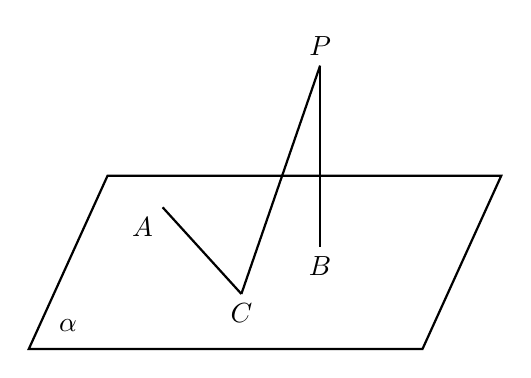
\begin{tikzpicture}[>=stealth, scale=1.0]
  % 平面 alpha
  \coordinate (M1) at (-0.5, -0.4);
  \coordinate (M2) at (4.5, -0.4);
  \coordinate (M3) at (5.5, 1.8);
  \coordinate (M4) at (0.5, 1.8);
  \draw[thick] (M1) -- (M2) -- (M3) -- (M4) -- cycle;
  \node at (0.0, -0.1) {$\alpha$};

  % 点坐标
  \coordinate (A) at (1.2, 1.4);
  \coordinate (B) at (3.2, 0.9);
  \coordinate (P) at (3.2, 3.2);
  \coordinate (C) at (2.2, 0.3);

  % 线段
  \draw[thick] (P) -- (B);
  \draw[thick] (P) -- (C);
  \draw[thick] (A) -- (C);

  % 节点标注
  \node[above] at (P) {$P$};
  \node[below] at (B) {$B$};
  \node[below left] at (A) {$A$};
  \node[below] at (C) {$C$};
\end{tikzpicture}
